




\chapter{Reflexions sobre la informació en la multiresolució}
\label{sec:multiresolucio:teoriainformacio}



En aquest capítol reflexionem sobre el problema d'identificar la
informació que selecciona un esquema de multiresolució i per tant
també d'observar quina informació no queda emmagatzemada i es perd.
Així doncs, cal estudiar l'aplicació de la teoria de la informació per
a l'esquema de multiresolució.  

En aquest context, els \gls{SGSTM} són un sistemes que emmagatzemen
les dades comprimides amb pèrdua d'una certa part de la informació
original. Aleshores, les consultes que es resolguin a partir d'un
\gls{SGSTM} són consultes aproximades a la informació total original,
llevat que mitjançant una anàlisi determinem que poden oferir
consultes exactes. A continuació reflexionem sobre com analitzar
l'error de les consultes de multiresolució respecte a la informació
original:
\begin{itemize}
\item Primer, descrivim de forma molt genèrica la teoria de la
  informació, la qual està relacionada amb la quantificació de la
  informació.
\item Segon, definim el problema de calcular l'error en la multiresolució.
\item Tercer, mostrem exemples d'anàlisi de la informació per alguns
  esquemes de multiresolució.
\end{itemize}



\todo{canviar subseccions a seccions}


\subsection{Teoria de la informació}

En altres àmbits, la teoria de la informació (\emph{information
  theory}) és el referent per a formalitzar la quantificació de la
informació. És també el cas de la compressió de dades, un àmbit proper
als \gls{SGSTM} en aquest context d'informació.  Per al cas particular
de compressió amb pèrdua s'aplica un subconjunt de la teoria anomenat
teoria de la taxa de
bit-distorsió %optimot: rate-distortion relationship
(\emph{rate–distortion theory}); la qual modela la percepció de la
distorsió i valora l'estètica dels resultats.


Per a quantificar la informació d'unes dades s'utilitza l'entropia, la
qual mesura la incertesa de predir els valors de les dades. Així, com
més entropia més aleatòries són les dades i com menys, més
redundants. Si l'entropia és zero aleshores les dades són totalment
predictible; és a dir donat un valor es coneix exactament quin és el
següent.




La compressió redueix la mida original de les dades. En el cas de la
compressió sense pèrdua es conserva la informació però s'augmenta
l'entropia, és a dir que s'elimina la redundància de les dades, i en
el cas de la compressió amb pèrdua es descarta informació que es
considera no essencial, per exemple en una imatge detalls que l'ull
humà no pot apreciar, tot i que també poden transformar les dades a un
altre domini on es es percebi millor la informació, per exemple
treballar en el domini freqüencial del so per a operacions
d'equalització. Aquesta aplicació de la compressió amb pèrdua per tal
de representar millor les dades també es coneix amb el nom de
codificació perceptiva (\emph{perceptual encoding}).



Els mètodes de compressió amb pèrdua se solen usar per a compressió de
multimèdia. L'objectiu és aconseguir menys volum de dades però que
conservin la mateixa percepció que les originals, o fins i tot amb una
pèrdua de qualitat perceptible mentre compleixi amb els requisits de
l'aplicació que se li vol donar. Així doncs, la compressió de
multimèdia sovint requereix valorar la percepció humana, per tal de
valorar la qualitat de percepció humana s'utilitzen testos
subjectius com per exemple el test
ABX\todo{ref}.  %http://en.wikipedia.org/wiki/ABX_test

%  Lossy methods are most often used for compressing sound, images or videos. This is because these types of data are intended for human interpretation where the mind can easily "fill in the blanks" or see past very minor errors or inconsistencies – ideally lossy compression is transparent (imperceptible), which can be verified via an ABX test. http://en.wikipedia.org/wiki/ABX_test
% Flaws caused by lossy compression that are noticeable to the human eye or ear are known as compression artifacts.




\todo{information algebra}
\url{https://en.wikipedia.org/wiki/Information_algebra}

algebra of information, describing basic modes of information processing. Such an algebra involves several formalisms of computer science, which seem to be different on the surface: relational databases, multiple systems of formal logic or numerical problems of linear algebra. It 



% El procediment
% que se segueix és: comprimir, emmagatzemar, descomprimir i
% visualitzar.
% compressed data must be decompressed to use -> en els sgstm no? bé si vull veure tota la sèrie temporal sí que he de concatenar el que hi tinc i per tant es pot veure com una descompressió (al marge que hi pot haver una compressió/descompressió en els agregadors usats, per exemple si és un so emmatgatzemar la freqüència i després s'haurà de descomprimir a amplitud al llarg del temps).
% The design of data compression schemes involves trade-offs among various factors, including the degree of compression, the amount of distortion introduced (e.g., when using lossy data compression), and the computational resources required to compress and uncompress the data.
% * No hi ha descompressió. Els algoritmes de compressió amb pèrdua normalment van associats amb les tècniques de compressió/descompressió; és a dir que les dades s'emmagatzemen amb estructures intermitges, que ocupen menys mida, i que cal descomprimir per recuperar-les. En els cas dels SGSTM les dades s'emmagatzemen com a subsèries temporals en els discs i per tant a l'hora de recuperar-les ja són sèries temporals, com a molt potser fa falta concatenar-les per a obtenir tota la sèrie temporal.



% The main drawback of lossy compression techniques is that they
% rely on specific patterns for providing a good approximation of the given time series.
% This is the main reason why lossy compression has been rarely applied to network
% monitoring contexts, where the patterns of time series can drastically change due to
% anomalous events or to transient networking issues.

%http://www.data-compression.com/theory.shtml


\subsection{Error en la informació de la multiresolució}

El model dels \gls{SGSTM} es basa en una compressió amb pèrdua, és a
dir descartar dades i emmagatzemar només aquella informació que es
consideri necessària o suficient. Així doncs, cal quantificar quin
error hi ha entre la informació emmagatzemada i la informació que
contenen les dades originals.


El problema genèric de la informació en la multiresolució és el següent.
\begin{definition}[Error en la informació de la multiresolució]
  Sigui una sèrie temporal $S$ i una sèrie temporal multiresolució $M$
  resultant de l'emmagatzematge i consolidació de $S$. De la sèrie
  temporal multiresolució es pot consultar la sèrie temporal total
  $S'=\glssymbol{not:sgstm:serietotal}(M)$, o bé de forma equivalent
  com s'ha vist abans\todo{ara és un capítol}
  $S'=\glssymbol{not:sgstm:multiresolucio}(S,e)$ on $e$ és l'esquema
  de $M$.  S'executa una operació de consulta $o$ sobre la sèrie
  temporal original $r_1=o(S)$ i la mateixa operació sobre la sèrie
  temporal de la multiresolució $r_2=o(S')$ . Es pot avaluar l'error
  de multiresolució $\epsilon=d(r_1,r_2)$ on $d$ és una funció que
  permet avaluar la distància entre els dos resultats, per exemple
  mínims quadrats si els resultats són sèries temporals \todo{ref?}.
\end{definition}


Cal aclarir que es podria avaluar $d(S,S')$, però aquest no és el
problema que intenten resoldre els \gls{SGSTM}. Aquest seria un
problema d'aproximació al senyal original, el qual altres models poden
resoldre més bé (per exemple last01 o ogras06?)\todo{ref?}. En canvi els \gls{SGSTM} resolen un
problema de compressió amb pèrdua per a seleccionar una determinada
informació.




En la informació de la multiresolució cal pensar també amb consultes
qualitatives. Per exemple una consulta podria ser $o=$`Creix la sèrie
temporal?' Aleshores no hi hauria error $\epsilon=d(r_1,r_2)$ quan la
resposta fos la mateixa per als dos casos, $r_1$ i $r_2$.


Tot i que hem proposat d'aplicar la mateixa operació $o$ a la
sèrie temporal original $r_1=o(S)$ i a la sèrie temporal de la
multiresolució $r_2=o(S')$, pot ser que l'operació hagi de ser
diferent per a obtenir el mateix resultat. És a dir $r_1=o(S)$ però
$r_2=o'(S')$ on $o'$ és l'operació equivalent a $o$ per aplicar
després de la multiresolució.  Per exemple, una operació $o$ podria
ser el càlcul de la multiresolució,
$r_1=\glssymbol{not:sgstm:multiresolucio}(S,e)$, aleshores l'operació
$o'$ equivalent és la identitat perquè el \gls{SGSTM} ja ha calculat
la multiresolució, $r_2=S'$ on $o'$ no hi és. Aquest exemple, de fet,
és el cas de la funció de multiresolució de la
\autoref{sec:multiresolucio:funcio}, on és equivalent l'operació de
multiresolució aplicada als \gls{SGST} que la sèrie temporal
emmagatzemada en un \gls{SGSTM}; per tant l'error
$\epsilon =d(r_1,r_2)$ seria nul.



Així doncs, l'error en la informació de la multiresolució permet
quantificar la pèrdua d'informació dels \gls{SGSTM}. Un cop
quantificat l'error per a un determinat esquema de multiresolució es
pot saber per a quines consultes serà apropiat aquell esquema i per a
quines no. Per a quantificar aquest error es poden preveure diversos
contextos:
\begin{itemize}
\item Hi ha consultes que es poden resoldre a la perfecció, és a dir
  sense error. Per exemple és el cas descrit on l'operació que es vol
  fer a una sèrie temporal és precisament la consulta de
  multiresolució.
  %altres exemples, per exemple en el cas de comptadors per a consultar totals

\item Es pot calcular l'error mesurant la diferència entre la mateixa
  consulta aplicada a les dades originals que a les dades
  emmagatzemades en el \gls{SGSTM}.

\item Es pot mesurar l'error mitjançant la visualització de les
  dades. És a dir, de manera semblant a la compressió amb pèrdua de
  multimèdia, l'usuari valora subjectivament si visualitza la mateixa
  informació en les dades originals com en les dades comprimides amb
  multiresolució. Per exemple, un dels criteris que recomana RRDtool
  per a establir un esquema és tenir en compte l'amplada de la
  pantalla on es visualitzen els resultats: no cal treballar amb una
  sèrie temporal amb molta resolució si no és possible observar-la
  \todo{ref}.
  % RRDtool expliquen un criteri que és definir les k dels discs inferior a l'amplada en píxels de la pantalla. Aquest és un criteri basat en una consulta per a fer visualització immediatament. Llavors no té sentit tenir més nombre de dades que les que es poden visualitzar.  Per exemple si capturem dades cada 5 minuts al llarg d'un any obtenim 43800 punts; si no disposem d'un monitor amb aquest nombre de píxels d'amplada no els podrem percebre.
  %Això potser també té relació amb el camp de gràfics 3D, on la multiresolució s'aplica per a no treballar amb objectes que només seran percebuts com un píxel?

\end{itemize}













\subsection{Exemples}

A continuació mostrem alguns exemples per tal de quantificar la
selecció o pèrdua d'informació que hi pot haver en un \gls{SGSTM}.


\begin{example}[Mateixa consulta i funció d'agregació d'atributs per a
  tota la sèrie temporal]
  \label{ex:multiresolucio:f=op}
  Sigui $S=\{m_0,\dotsc,m_k\}$ una sèrie temporal, on $m_k=(t_k,v_k)$,
  i $e= \{ (\delta_0, f_0, \tau_0, k_0) \}$ un esquema de
  multiresolució amb una sola subsèrie resolució, suposem $k_0=\infty$
  per tal de negligir-ne l'efecte i $\tau_0=T(\min(S))$. Obtenim la
  sèrie temporal resultant d'aplicar la funció de multiresolució
  $S'=\glssymbol{not:sgstm:multiresolucio}(S,e)$.  Així, aquesta sèrie
  temporal resultant contindrà mesures calculades a partir de
  l'agregació de $S$ en els intervals definits per $\tau_0$ i
  $\delta_0$ i tindrà la forma $S'=\{ f_0(S,[\tau_0,\tau_0+\delta_0],
  f_0(S,[\tau_0+\delta_0,\tau_0+2\delta_0]),\dotsc,
  f_0(S,[\tau_0+(M-1)\delta_0,\tau_0+M\delta_0])\}$ on
  $\tau_0+M\delta\geq T(\max(S))$ i $M\in\glssymbol{not:N}$. Si
  escrivim de forma genèrica $v_0,\dotsc,v_{i_1}$ els valors originals
  usats en l'agregació del primer interval
  $f_0(S,[\tau_0,\tau_0+\delta_0])$, $v_{i_1+1},\dotsc,v_{i_2}$ els del
  segon interval, etc. aleshores podem expressar $S'=\{
  (\tau_0+\delta_0, f'(v_0,\dotsc,v_{i_1})), (\tau_0+2\delta_0,
  f'(v_{i_1+1},\dotsc,v_{i_2})), \dotsc, ((\tau_0+M\delta_0 ,f'(v_{i_M},
  \dotsc, v_k)) \}$ on $f'$ és l'aplicació corresponent de l'atribut
  que resumeix $f_0$.

  Apliquem un operador de consulta $o$ a les dues sèries temporals,
  $r_1=o(S)$ i $r_2=o(S')$, que és la mateixa funció d'agregació
  d'atributs de l'esquema multiresolució però aplicat a tots els
  valors de la sèrie temporal,
  $o(S)=V(f_0(S,[-\infty,\infty]))$. Analitzem els efectes segons dues
  funcions d'agregació d'atributs:

  \begin{itemize}
  \item Màxim: $f_0=\glssymbol{not:sgstm:maxdd}$, segons definit al
    model de \gls{SGSTM}, el qual si negligim l'atribut de temps es
    correspon a aplicar l'agregació $o=\glssymbol{not:sgst:maxv}$,
    segons definit al model de \gls{SGST}, i per tant a calcular
    l'atribut $f'=\max$ dels valors.

    Si $S=\{m_0,\dotsc,m_k\}$ on $m_k=(t_k,v_k)$ aleshores
    $r_1=o(S)=\max(v_0,\dotsc, v_k)$. En canvi $S'=\{
    (\tau_0+\delta_0, \max(v_0,\dotsc,v_{i_1})),
    (\tau_0+2\delta_0,\max(v_{i_1+1},\dotsc,v_{i_2})), \dotsc,
    (\tau_0+M\delta_0,\max(v_{i_M}, \dotsc, v_k)) \}$ i aleshores
    $r_2=o(S')= \max\big( \max(v_0,\dotsc,v_{i_1}),
    \max(v_{i_1+1},\dotsc,v_{i_2}), \dotsc, \max(v_{i_M}, \dotsc v_k)
    \big)$.

    Podem concloure que en aquest cas $r_1=r_2$, i per tant
    $\epsilon=d(r_1,r_2)=0$ , perquè $\max(v_0,\dotsc, v_k) =
    \max\big( \max(v_0,\dotsc,v_{i_1}),
    \max(v_{i_1+1},\dotsc,v_{i_2}), \dotsc, \max(v_{i_M}, \dotsc v_k)
    \big)$ i $\max$ és una funció associativa: $\max(a,b,c,d,e) = \max(
    \max(a,b), \max(c,d,e))$.

    En aquest exemple hem negligit els temps resultants de
    l'agregació. És a dir, $r_1$ és correspon amb una o més d'una
    mesura $m_a\in S: V(m_a)=r_1$ i de la mateixa manera $m_b\in S':
    V(m_b)=r_2$ on hem conclòs que $V(m_a)=V(m_b)$. Això no obstant,
    en general els temps d'aquestes mesures no es correspondran,
    $T(m_a)\neq T(m_b)$ perquè $f_0=\glssymbol{not:sgstm:maxdd}$
    resumeix els atributs de temps segons l'interval de consolidació i
    al marge del resum de la informació en els valors.



\item   Mitjana aritmètica:
  $f_0=\glssymbol{not:sgstm:mitjanadd}$\todo{NOOOO} la mitjanadd
  divideix per tf-t0, cal una mitjana que divideixi pel
  cardinal!!!!!\todo{noo: ha de ser la mitjanaParcial el que de moment
    es diu mitjana aritmètica$^d$}, segons definit al model de
  \gls{SGSTM}, el qual si negligim l'atribut de temps es correspon a
  aplicar l'agregació $o=\glssymbol{not:sgst:mitjanav}$, segons
  definit al model de \gls{SGST}, i per tant a calcular l'atribut
  $f'=\operatorname{mitjana}$ (aritmètica) dels valors.

    De manera similar al cas anterior, els resultats són
    $r_1=\operatorname{mitjana}(v_0,\dotsc, v_k)$ i
    $r_2=\operatorname{mitjana}\big(
    \operatorname{mitjana}(v_0,\dotsc,v_{i_1}),
    \operatorname{mitjana}(v_{i_1+1},\dotsc,v_{i_2}), \dotsc,
    \operatorname{mitjana}(v_{i_M}, \dotsc v_k) \big)$.  Però en
    aquest cas hem de concloure que $\epsilon=d(r_1,r_2)\geq 0$ perquè
    la mitjana no és una funció associativa:
    $\operatorname{mitjana}(a,b,c,d,e) \neq \operatorname{mitjana}(
    \operatorname{mitjana}(a,b), \operatorname{mitjana}(c,d,e))$.
 


  \item Total: definim una funció d'agregació d'atributs
    $f_0=\operatorname{total}$ que, negligint l'atribut de temps,
    resumeix la sèrie temporal amb la suma dels valors:
    $\operatorname{total}: S \times [t_a,t_b] \mapsto m'$ i $V(m') =
    \sum\limits_{\forall m\in S(t_a,t_b]} V(m)$. Així doncs, es
    correspon a calcular $o=\glssymbol{not:sgst:sumav}$, segons
    definit al model de \gls{SGST}, i per tant a calcular l'atribut
    $f'=\sum$ dels valors.

    Aquest cas és similar al del màxim, $r_1=\sum(v_0,\dotsc, v_k)$ i
    $r_2=\sum\big( \sum(v_0,\dotsc,v_{i_1}),
    \sum(v_{i_1+1},\dotsc,v_{i_2}), \dotsc, \sum(v_{i_M}, \dotsc v_k)
    \big)$, i $\epsilon=d(r_1,r_2)=0$ perquè la suma és una funció
    associativa.
    



  \end{itemize}

$\square$
\end{example}






\begin{example}[Mitjana per a una sèrie temporal regular]
  Seguint l'\autoref{ex:multiresolucio:f=op}, podem estudiar en quins
  casos la mitjana aritmètica no té error. Com ja s'ha dit, la mitjana
  no és una funció associativa. Però sí que esdevé associativa quan
  s'associen el mateix nombre d'elements:
  $\operatorname{mitjana}(a,b,c,d,e,f) = \operatorname{mitjana}(
  \operatorname{mitjana}(a,b), \operatorname{mitjana}(c,d),
  \operatorname{mitjana}(e,f)) = \operatorname{mitjana}(
  \operatorname{mitjana}(a,b,c), \operatorname{mitjana}(d,e,f))$.

  Per tal que s'associïn el mateix nombre d'elements cal que per cada
  interval de consolidació de la sèrie temporal hi hagi el mateix
  nombre de mesures:
  $|S[\tau_0,\tau_0+\delta_0]|=|S[\tau_0+\delta_0,\tau_0+2\delta_0]|=\dotsb
  = |S[\tau_0+(M-1)\delta_0,\tau_0+M\delta_0]|$.  Aquest cas es
  compleix, per exemple, quan la sèrie temporal és regular amb període
  $d$ i el pas de consolidació de l'esquema multiresolució és múltiple
  de la regularitat de la sèrie temporal, $\delta_0 = nd$ on
  $n\in\glssymbol{not:N}$, o bé quan la sèrie temporal és de temps
  real amb període $d$ i iniciada a $t_I$ i la multiresolució n'és
  múltiple: $\delta_0 = nd$ i $\tau_0 = t_I+n\delta$ (v.\ secció de
  regularitat de la sèrie temporal\todo{ref}).

  Aleshores, en aquest casos, sí que es podria concloure que
  $\epsilon=d(r_1,r_2)=0$ per la multiresolució amb mitjana.
\end{example}





\begin{example}[Consultes per a un interval determinat]
\label{ex:multireoslucio:informacio-subresolucions}

En l'\autoref{ex:multiresolucio:f=op} l'operació de consulta $o$
s'aplica a tota la sèrie temporal $S[-\infty,\infty]$. Ara plantegem
d'aplicar-la a un interval concret de la sèrie temporal $S[t_a,t_b]$
on $t_a$ i $t_b$ són dos instants de temps.  Analitzem quan l'interval
$[t_a,t_b]$ és múltiple dels intervals de multiresolució consolidats,
$t_a=\tau_0+n\delta_0$ i $t_b=\tau_0+(n+l)\delta_0$ on
$n,l\in\glssymbol{not:N}$, i quan no ho és:

\begin{itemize}
\item L'interval és múltiple dels intervals de multiresolució
  consolidats. Aleshores $r_1=V(f_0(S,[t_a,t_b]))$,
  $r_2=f_0(S',[t_a,t_b])$ on $S'= \{ \dotsc, (t_a,
  f'(v_{i_a},\dotsc,v_{i_a+1}) ), \dotsc, (t_b,
  f'(v_{i_b-1},\dotsc,v_{i_b})), \dotsc \}$ i
  $v_{i_a},\dotsc,v_{i_a+1}$ són els valors de les mesures en
  $S[t_a,t_a+\delta_0]$ i $v_{i_b-1},\dotsc,v_{i_b}$ en
  $S[t_b-\delta_0,t_b]$.

  Per tant, per a estudiar $d(r_1,r_2)$ se segueix analitzant el
  comportament de la funció de resum de l'atribut per als dos casos
  $r_1=f'(v_{i_a},\dotsc,v_{i_a+1},\dotsc, v_{i_a+1},\dotsc,v_{i_b})$
  i $r_2=f'(f'(v_{i_a},\dotsc,v_{i_a+1}),\dotsc,
  f'(v_{i_a+1},\dotsc,v_{i_b}))$ de la mateixa manera que a 
  l'\autoref{ex:multiresolucio:f=op}.


\item L'interval no és múltiple dels intervals de multiresolució
  consolidats.  Per a simplificar la notació, suposem $t_a=\tau_0$ i
  $\tau_0+\delta < t_b \leq \tau_0+2\delta_0$.  Aleshores
  $r_1=V(f_0(S,[t_a,t_b]))$, $r_2=f_0(S',[t_a,t_b])$ on $S'=
  \{(\tau_0+\delta, f'(v_{i_0},\dotsc,v_{i_1}) ),(\tau_0+2\delta ,
  f'(v_{i_1+1},\dotsc,v_{b} ,\dotsc,v_{i_2})), \dotsc \}$ on els
  valors s'anoten com a l'\autoref{ex:multiresolucio:f=op} i $v_b$
  assenyala una possible mesura en l'instant $t_b$.  A la
  \autoref{fig:multiresolucio:informacio-subresolucions} es mostra els
  instants de temps i els valors d'aquest exemple, l'interval
  temporal $[t_a,t_b]$ de la consulta i l'interval temporal
  $[t_b,\tau_0+2\delta_0]$ que mostra l'error en la consulta a partir
  de la informació emmagatzemada a la multiresolució.


\begin{figure}[tp]
  \centering
     \begin{tikzpicture}
        \begin{axis}[
          ymin = 0,
          yticklabels= {},
          xticklabels={,,$\underset{t_a}{\tau_0}$,,$\tau_0+\delta$,$t_b$,$\tau_0+2\delta$},
          ]
          \addplot[ycomb,blue] coordinates {
            (20,10)
            (30,10)
            (40,10)
          }; 
          
 
          \addplot[
          ybar interval, 
          fill=green!25,
          fill opacity=0.5,
          draw=none,
          ] plot coordinates
          {(20,7)(35,7)};

          \addplot[
          ybar interval, 
          fill=orange!75,
          fill opacity=0.5,
          draw=none,
          ] plot coordinates
          {(35,7)(40,7)};


          \addplot[red,mark=*,only marks] coordinates {
            (20,2)
            (30,2)
            (35,2)
            (40,2)
          }; 


          \node[right] at (axis cs:37,5) {$\epsilon$};

          \node[right] at (axis cs:20,3) {$v_{i0}$};
          \node[right] at (axis cs:30,3) {$v_{i1}$};
          \node[right] at (axis cs:30,4) {$v_{i1+1}$};
          \node[right] at (axis cs:35,3) {$v_{b}$};
          \node[left] at (axis cs:40,3) {$v_{i2}$};
        \end{axis}
      \end{tikzpicture}

      \caption{Sèrie temporal amb la consulta desitjada (verd) i l'error de la
        informació no coneguda (taronja)}
  \label{fig:multiresolucio:informacio-subresolucions}
\end{figure}




  Cal tenir en compte que $f_0(S',[t_a,t_b])$ ha de resoldre la
  selecció en l'interval: 
  \begin{enumerate}
  \item amb una selecció d'interval $S'[t_a,t_b]=\{ (\tau_0+\delta,
    f'(v_{i_0},\dotsc,v_{i_1}) ) \}$,

  \item amb una selecció d'interval temporal
    $S'[t_a,t_b]^r=(\tau_0+\delta, f'(v_{i_0},\dotsc,v_{i_1}), (t_b,
    f^r(f'(v_{i_1+1},\dotsc,v_{b} ,\dotsc,v_{i_2}))) ) $ on $f^r$ és
    la interpolació realitzada per la funció de representació $r$

  \item o amb altres casos, podem pensar per exemple
    $S'[t_a,t_b]^r=(\tau_0+\delta, f'(v_{i_0},\dotsc,v_{i_1}), (t_b,
    f'(v_{i_1+1},\dotsc,v_{b} ,\dotsc,v_{i_2})) )$.
   \end{enumerate}



  Així, per a estudiar $\epsilon=d(r_1,r_2)$ s'ha d'analitzar
  $r_1=f'(v_{i_0},\dotsc,v_{i_1},\dotsc, v_{i_1+1},\dotsc,v_{b})$ i,
  depenent de la selecció,
   \begin{enumerate}
   \item $r_2=f'(f'(v_{i_0},\dotsc,v_{i_1}))$, 

   \item
     $r_2=f'(f'(v_{i_0},\dotsc,v_{i_1}),f^r(f'(v_{i_1+1},\dotsc,v_{b},\dotsc,v_{i_2})))$
     \item o $r_2=f'(f'(v_{i_0},\dotsc,v_{i_1}),f'(v_{i_1+1},\dotsc,v_{b},\dotsc,v_{i_2}))$.
\end{enumerate}

  És a dir, en la multiresolució consolidada no hi ha disponible la
  informació $f'(v_{i_1+1},\dotsc,v_{b})$ que es voldria consultar.
  Per tant hem de concloure que generalment $\epsilon=d(r_1,r_2)\geq
  0$ quan l'interval consultat no és múltiple de la resolució
  emmagatzemada, tret que coneguéssim exactament el comportament de la
  sèrie temporal i poguéssim determinar la funció de representació que complís 
  $ f'(v_{i_1+1},\dotsc,v_{b}) = f^r(f'(v_{i_1+1},\dotsc,v_{b},\dotsc,v_{i_2}))$.
\end{itemize}


Així doncs, hi haurà un cert error en el cas que els intervals
consultats no siguin múltiples de la multiresolució emmagatzemada:
seguint l'exemple, caldria calcular $f'(v_{i_1+1},\dotsc,v_{b})$ però
la informació que hi ha emmagatzemada per a aquest interval és
$f'(v_{i_1+1},\dotsc,v_{b},\dotsc,v_{i_2})$. Estudiem dos dels
atributs descrits a l'\autoref{ex:multiresolucio:f=op} per tal
d'avaluar si és possible afitar-ne error en aquests casos:

\begin{itemize}

\item Màxim. Cal calcular $\max(v_{i_1+1},\dotsc,v_{b})$ però hi ha
  emmagatzemat $\max(v_{i_1+1},\dotsc,v_{b},\dotsc,v_{i_2})$.  Per
  tant l'error en la consulta és $\epsilon=d(r_1,r_2)=
  d(\max(v_{i_1+1},\dotsc,v_{b}),\max(v_{i_1+1},\dotsc,v_{b},\dotsc,v_{i_2}))$. Si
  el màxim es troba a $[t_a+\delta_0,t_b]$ l'error és nul però si hi
  ha un màxim a $[t_b,t_a+2\delta_0]$ aleshores l'error és
  $\epsilon=d(\max(v_{i_1+1},\dotsc,v_{b}),\max(v_{b},\dotsc,v_{i_2}))$,
  el qual no és fitable.
  
\item Total: Cal calcular $\sum(v_{i_1+1},\dotsc,v_{b})$ però hi ha
  emmagatzemat $\sum(v_{i_1+1},\dotsc,v_{b},\dotsc,v_{i_2})$. Per tant
  l'error en la consulta és $\epsilon=d(r_1,r_2)=d(
  \sum(v_{i_1+1},\dotsc,v_{b},\dotsc,v_{i_2}),\sum(v_{i_1+1},\dotsc,v_{b}))
  = \sum(v_{b+1},\dotsc,v_{i_2})$. Però $\sum(v_{b+1},\dotsc,v_{i_2})$
  no és un valor emmagatzemat a la multiresolució i per tant no es pot
  saber l'error. Això no obstant, en el cas del total té sentit
  plantejar el cas que la variable mesurada és monòtona creixent
  (v.~\autoref{ex:multiresolucio:comptadors}): aleshores es compleix
  que $\sum(v_{i_1+1},\dotsc,v_{b}) \leq
  \sum(v_{i_1+1},\dotsc,v_{b},\dotsc,v_{i_2})$ i per tant es pot fitar
  l'error $\epsilon=d(r_1,r_2) = \sum(v_{b+1},\dotsc,v_{i_2}) \leq  
  \sum(v_{i_1+1},\dotsc,v_{b},\dotsc,v_{i_2})$; és a dir com a màxim
  es cometria un error del valor consolidat a $\tau_0+2\delta$ que
  significaria que en els pitjors del casos tota la mesura hauria
  ocorregut després de $t_b$.


\end{itemize}




\end{example}











\begin{example}[Aplicació de la conservació de la mitjana de la funció
  en comptadors]
  \label{ex:multiresolucio:comptadors}

  Aquest exemple prové d'una reflexió acurada de per què RRDtool té
  com a referent els comptadors.



%\todo{parlar de comptadors monòtons creixents?? o de comptadors en general}

  Un comptador monòton creixent és un aparell que mesura l'energia en
  un determinat interval de temps. Entre dues lectures successives del
  comptador la mesura de l'energia és exacta a diferència d'un aparell
  que mesuri potència instantània, de la qual només es pot deduir
  l'energia exacta si es considera que el senyal es pot reconstruir:
  per exemple compleix Nyquist\todo{ref} tot i que a la pràctica és
  complicat conèixer la freqüència de les variables mesurades atès que
  solen ser aleatòries o canvien bruscament. A la inversa també ocorre
  el mateix, a partir de la mesura de l'energia només es pot deduir la
  potència instantània exacta si es considera que el senyal es pot
  reconstruir.  Els conceptes d'energia i potència solen anar
  associats a un determinat tipus de variables físiques contínues; en
  altres comptadors els conceptes equivalents són el quantitat,
  comptatge total o increments per a l'energia i el flux o la
  velocitat per a la potència.


% ha d'aparèixer potència mitjana (que és la línia) i energia (que és l'àrea sota la línia). els aparells tant poden mesurar en un interval energia com potència mitjana i és el mateix, si la mesura mitjana és real i no a partir de la mitjana de diverses instantànies. 

  No totes les variables físiques són susceptibles de ser mesurades
  amb un comptador. Els comptadors es poden aplicar per exemple per a
  mesurar energia elèctrica, aforaments de trànsit en una carretera, consum
  d'aigua, etc.
  
  \todo{dir que} a l'exemple 2.19 %\autoref{ex:sgst:comptador-electricitat}
 del model sgst hi ha un exemple de sèrie temporal per a la mesura de potència i energia elèctrica 


  En resum, l'aparell condiciona la informació que es podrà extreure
  de la mesura; en aquest exemple ens centrem en la informació de
  l'energia i de quina manera la multiresolució és capaç de conservar
  exactament algunes propietats d'aquesta informació.  Per a aquest
  exemple suposem aparells de mesura ideals quan parlem de mesura
  exacta; és a dir que no tenim en compte l'error de precisió o
  d'exactitud de l'aparell.

 



\begin{figure}[tp]
  \centering

     \begin{tikzpicture}
        \begin{axis}[
          title={$E(t)=\int P(t) dt$},
          ymin=0,
          ymax=3,
          xmax=21,
          domain=0:20,
          ylabel=$P(t)$,
          xlabel=$t$,
          xtick=\empty,
          ytick=\empty,
          axis x line=left,
          axis y line=left,
          ]

          % \addplot[const plot, blue,fill=blue,smooth,
          % ] plot coordinates
          % {(0,4)(1,2)(2,6)(3,4)(4,4)};


          \addplot[pattern=crosshatch dots, pattern
          color=blue,draw=blue, samples=500] {2+sin(deg(x))/2} \closedcycle;



          \node at (axis cs:10,1) {$E(t)$};


     \end{axis}
      \end{tikzpicture}  

      \caption{Relació entre l'energia i la potència o la quantitat
        comptada i la velocitat}
  \label{fig:multiresolucio:energia-potencia}
\end{figure}




Així doncs, la definició del problema és la següent.  Sigui $E(t)$
l'energia d'un senyal i $P(t)$ la potència instantània del senyal, es
compleix la relació $E(t)=\int P(t) dt$, que es mostra a la
\autoref{fig:multiresolucio:energia-potencia}; que és la mateixa
relació $Q(t)=\int v(t) dt$ per a un comptador on $Q$ és la quantitat
comptada i $v$ és la velocitat instantània, o la mateixa per a un cas
discret $\Delta Q = \bar{v} \Delta t$ on $\bar{v}$ és la velocitat
mitjana mesurada durant $\Delta t$. %
  %Potser el cas discret hauria de ser $\Delta Q = \sum \bar{v}_k \Delta t_k$
  Siguin
  $[t_a,t_b]$ i $[t_b,t_c]$ dos intervals de temps de mesura, un
  comptador mesura exactament el valor de $\int_{t_a}^{t_b} P(t)$ i de
  $\int_{t_b}^{t_c} P(t)$. En canvi, un aparell de mesura de potència
  instantània es capaç de mesurar exactament $P(t_a)$, $P(t_b)$ i
  $P(t_c)$. Ara bé, a partir del comptador no es poden deduir
  exactament $P(t_a)$, $P(t_b)$ ni $P(t_c)$ i a partir de la mesura de
  la potència instantània no es poden deduir exactament
  $\int_{t_a}^{t_b} P(t)$ ni $\int_{t_b}^{t_c} P(t)$. Tampoc a partir
  del comptador es poden deduir exactament energies que no s'han
  mesurat, per exemple ni $\int_{(t_a+t_b)/2}^{t_b} P(t)$ ni
  $\int_{(t_a+t_b)/2}^{t_c} P(t)$; ara bé sí que serà exacte el càlcul
  $\int_{t_a}^{t_b} P(t)+\int_{t_b}^{t_c} P(t)$.
  

  La multiresolució és capaç de conservar aquesta exactitud del
  comptatge total.  El comptatge total es pot conservar amb una
  multiresolució amb funcions d'agregació per atributs de suma de
  totals o bé per atributs de mitjana de la funció. Aquests darrers
  són els que permeten a més expressar la sèrie temporal resultant de
  la multiresolució de forma més coherent amb l'original (vegeu secció
  de naturalesa de comptadors \todo{ref}). Reprenent
  l'\autoref{ex:multiresolucio:f=op}, avaluem els atributs de mitjana
  de la funció, els quals són semblants als atributs de total però
  considerant la sèrie temporal en la representació contínua:
  
  \begin{itemize}

  \item Mitjana de la funció:
    $f_0=\operatorname{mitjana}^c$\todo{operador no declarat a la
      taula}, segons definit al model de \gls{SGSTM}, el qual si
    negligim l'atribut de temps es correspon a calcular la mitjana
    de la funció de representació de la sèrie temporal $\frac{1}{b-a}
    \int_{a}^{b} S(t)dt$ en l'interval tancat $[a,b]$.

    Sigui $t_M=T(\max(S)$ i $t_m=T(\min(S))$ i $S'= \{
    (\tau_0+\delta_0, \frac{1}{\delta_0}
    \int_{\tau_0}^{\tau_0+\delta_0} S(t) dt), (\tau_0+2\delta_0,
    \int_{\tau_0+\delta_0}^{\tau_0+2\delta_0} S(t) dt), \dotsc,
    (\tau_0+M\delta_0, \frac{1}{\delta_0}
    \int_{\tau_0+(M-1)\delta_0}^{\tau_0+M\delta_0} S(t) dt \}$, on
    s'ha aplicat $\delta_0= (\tau_0+\delta_0)-(\tau_0)=\dotsb=
    (\tau_0+M\delta_0)-(\tau_0+(M-1)\delta_0)$.  Els resultats que cal
    calcular són $r_1=\frac{1}{t_M-t_m} \int_{t_m}^{t_M} S(t)dt$ i
    $r_2 = \frac{1}{t_M-t_m} \int_{t_m}^{t_M} S'(t)$.

    Si suposem $\tau_0=t_m$ i $\tau_0+M\delta_0=t_M$ aleshores
    $\int_{t_m}^{t_M} S'(t) = \int_{\tau_0}^{\tau_0+\delta_0} S'(t) dt + \int_{\tau_0+\delta_0}^{\tau_0+2\delta_0} S'(t) dt + \dotsb + \int_{\tau_0+(M-1)\delta_0}^{\tau_0+M\delta_0}
    S'(t) dt$.  
    
    Si resolem per exemple el primer interval de consolidació: $
    \int_{\tau_0}^{\tau_0+\delta_0} S'(t) dt = \delta_0V(m'_0) =
    \delta_0 \frac{ \int_{\tau_0}^{\tau_0+\delta_0} S(t)
      dt}{\delta_0}$ on $m'_0$ és la mesura corresponent a la
    consolidació en el primer interval. Així doncs
    $\int_{\tau_0}^{\tau_0+\delta_0} S'(t) dt =
    \int_{\tau_0}^{\tau_0+\delta_0} S(t) dt$, de fet és la propietat
    que resumeix la mitjana de la funció, i per tant podem estendre-ho
    a $\int_{t_m}^{t_M} S'(t)= \int_{t_m}^{t_M} S(t)$. Podem
    concloure, doncs, que $r_1=r_2$.


    A la \autoref{fig:multiresolucio:comptador} es mostra un exemple
    amb valors concrets on $S=\{ (1,4),(2,2),(3,6),(4,4)\}$, l'esquema
    de multiresolució és
    $e=\{\{(\delta,2),(f,\glssymbol{not:sgstm:meanzohe}),(\tau,0),(k,\infty)\}
    \}$,així la sèrie resultant de la consulta multiresolució
    és $S'=\{ (2,3),(4,5)\}$, i les sèries temporals es representen amb
    representació \gls{zohe}.


\begin{figure}[tp]
  \centering


     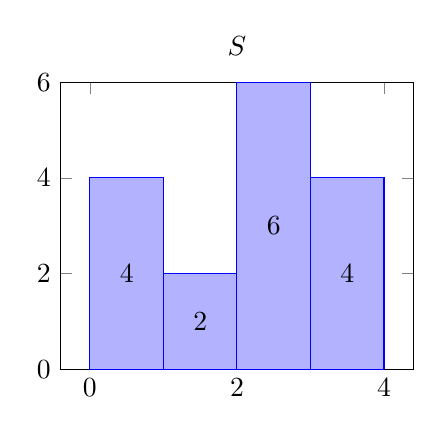
\begin{tikzpicture}
        \begin{axis}[
          width=0.5*\textwidth,
          title=$S$,
          ymin = 0,
          ymax=6,
          ]
          \addplot[
          ybar interval, 
          blue,fill=blue!30!white,
          ] plot coordinates
          {(0,4)(1,2)(2,6)(3,4)(4,4)};


    \node at (axis cs:0.5,2) {$4$};
    \node at (axis cs:1.5,1) {$2$};
    \node at (axis cs:2.5,3) {$6$};
    \node at (axis cs:3.5,2) {$4$};


     \end{axis}
      \end{tikzpicture}\qquad
     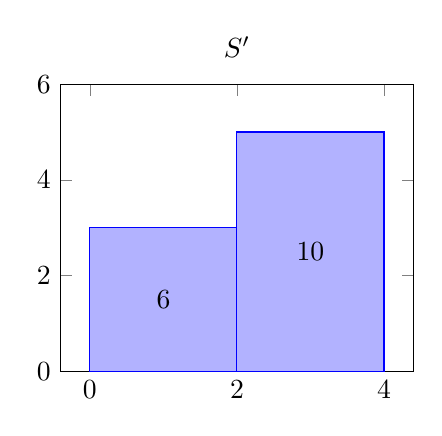
\begin{tikzpicture}
        \begin{axis}[
          width=0.5*\textwidth,
          title=$S'$,
          ymin = 0,
          ymax=6,
          ]

          \addplot[
          ybar interval, 
          blue,fill=blue!30!white,
          ] plot coordinates
          {(0,3)(2,5)(4,5)};

    \node at (axis cs:1,1.5) {$6$};
    \node at (axis cs:3,2.5) {$10$};


     \end{axis}
      \end{tikzpicture}


      \caption{Sèrie temporal amb àrea sota la corba i sèrie temporal
        resultant de la multiresolució amb agregació mitjana de la
        funció}
  \label{fig:multiresolucio:comptador}
\end{figure}






  \end{itemize}
  






  La multiresolució, però, no pot conservar la resolució del
  comptatge.  Com s'ha exposat a
  l'\autoref{ex:multireoslucio:informacio-subresolucions}, en
  consultes en què l'interval no es correspongui amb les resolucions
  emmagatzemades, els totals no seran els correctes que s'obtindrien
  de calcular amb les dades originals.  De fet, és el mateix problema
  que hem exposat que a partir d'un comptador no es poden deduir
  exactament energies que no s'han mesurat.


\end{example}

\todo{potser fer un exemple on es vegi com la multiresolució pot solucionar un problema d'inframostreig en els comptadors}




\begin{example}[Equivalències en l'agregació d'atributs]

  Hi ha casos en què és el mateix aplicar una funció d'agregació
  d'atributs que aplicar-ne una altra. Per exemple és el cas de la
  $\operatorname{mitjana}$\todo{falta definir a la taula} i el de la
  $\glssymbol{not:sgstm:meanzohe}$ per a sèries temporals regulars. 

  Sigui $S=\{m_0,\dotsc,m_k\}$, on $m_k=(t_k,v_k)$, una sèrie temporal
  regular de període $d$ i sigui $[t_a,t_b]$ un interval de temps on
  $t_a=T(\min(S))-d=t_0-d$ i $t_b=T(\max(S))=t_k$.  Demostrem que
  $\glssymbol{not:sgstm:meanzohe}(S,[t_a,t_b]) =
  \operatorname{mitjana}(S,[t_a,t_b])$.

  La mitjana aritmètica de la sèrie temporal és
  $\operatorname{mitjana}(S,[t_a,t_b])=\frac{v_0+\dotsb+v_k}{|S|}$
  
  La mitjana amb representació \gls{zohe} és
  $\glssymbol{not:sgstm:meanzohe}(S,[t_a,t_b])= \frac{1}{t_b-t_a} (
  v_0(t_0-t_a)+v_1(t_1-t_0)+\dotsb+ v_k(t_k-t_{k-1}) )$.

  Per ser regular, $t_1-t_0 = \dotsb = t_k-t_{k-1} = d$. A més
  $t_a=t_0-d$ i per tant $t_0-t_a = d$. També per ser regular,
  $t_k-t_0= t_k +(- t_{k-1} + t_{k-1}) + \dotsb + (- t_1 + t_1) - t_0
  = (|S|-1)d$ i per tant $t_b-t_a=t_k - (t_0 - d) = (|S|-1)d +d = |S|d$.

  Reescrivint, $\glssymbol{not:sgstm:meanzohe}(S,[t_a,t_b])=
  \frac{1}{|S|d} ( v_0d+v_1d+\dotsb+ v_kd ) = \frac{1}{|S|} (
  v_0+v_1+\dotsb+ v_k ) = \operatorname{mitjana}(S,[t_a,t_b])$.



  Així doncs, en una sèrie temporal regular es pot aplicar la
  $\operatorname{mitjana}$ com a equivalent a la
  $\glssymbol{not:sgstm:meanzohe}$; la
  \autoref{fig:multiresolucio:comptador} n'és un exemple. Un àmbit
  d'aplicació d'aquestes equivalències pot ser el de simplificar els
  càlculs en les consultes als \gls{SGSTM}, en els discs dels quals
  les subsèries temporals normalment s'emmagatzemen regulars.
  
\end{example}











%%% Local Variables:
%%% TeX-master: "main"
%%% End:

